\subsection{Les tests de base}

Les tests fournis passent tous avec succès dans l'implémentation dépourvue des
améliorations 'avancées' du sujet dont certaines sont en cours de
développement.

Des tests avec valgrind révèlent qu'il n'y a pas de fuite mémoire lors de
l'exécution de ces tests exception faite de ceux qui ne réalisent pas de
\verb!thread_join()! pour chaque thread créé via \verb!thread_create()!. C'est
le cas du test faisant un \verb!thread_join()! sur le main.

C'est un défaut qu'il nous est possible de corriger en testant la présence de
threads non joints à la fin du programme (via un destructeur) mais cela pourrait
entrer en conflit avec le code client qui pourrait potentiellement vouloir
faire la même chose. Nous avons donc choisi de laisser à l'utilisateur de la
bibliothèque le soin de terminer proprement chaque thread tout comme le fait
déjà pthread (les ressources ne sont libérées qu'après un \verb!pthread_join()!
pour les threads non détachés).

Nous avons également écrit un script pour tracer les courbes de performance
afin de pouvoir comparer graphiquement les temps d'exécution de notre
implémentation de threads utilisateurs lorsqu'on utilise les threads noyaux
et lorsqu'on ne les utilise pas.

\subsection{Tests implémentés}

\subsubsection{Les tris de tableaux} Les algorithmes de tri de tableaux $tri
rapide$ et $tri fusion$ ont été implémentées. Dans le cas du $tri rapide$
(fig. \ref{fig:quicksort}), un thread est créé et traite chaque partie du
tableau de part et d'autre du pivot. Pour le $tri fusion$
(fig. \ref{fig:mergesort}), chaque fois qu'un tableau est divisé en deux,
chaque partie est traitée par un nouveau thread.\\

%%%% resultats tests + include graphics %%%%
\begin{figure}[H]
\centering
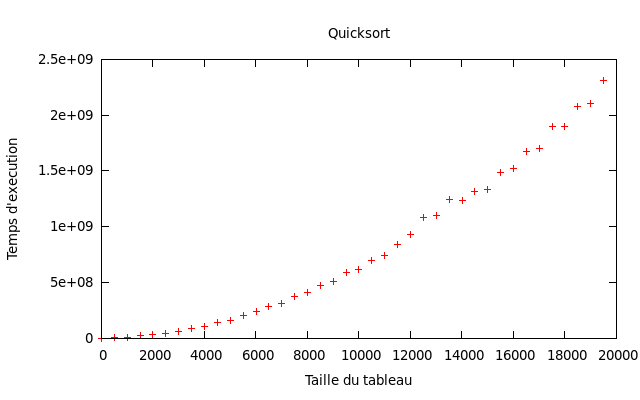
\includegraphics[width=0.9\textwidth]{quicksort.png}
\caption{Temps d'exécution des tests d'un tri rapide}
\label{fig:quicksort}
\end{figure}

%%%% resultats tests + include graphics %%%%
\begin{figure}[H]
\centering
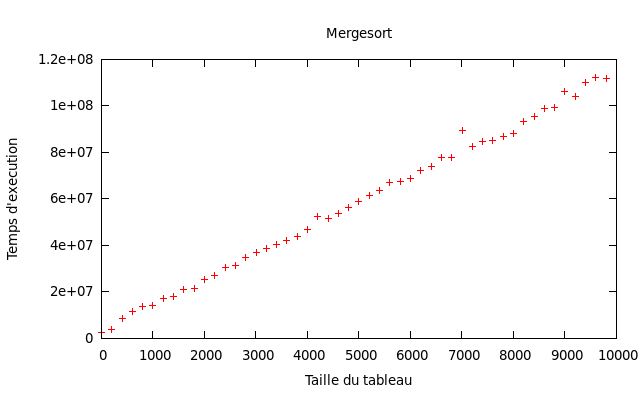
\includegraphics[width=0.9\textwidth]{mergesort.png}
\caption{Temps d'exécution des tests d'un tri fusion}
\label{fig:mergesort}
\end{figure}

\subsubsection{Somme des éléments d'un tableau} Pour calculer la somme des
éléments d'un tableau (fig. \ref{fig:arraysum}), nous utilisons le même principe que pour le tri fusion,
à savoir diviser le tableau en deux et attribuer les deux parties à des threads
distincts. Une fois que l'on obtient des tableaux d'une case, leur valeur est
retournée et le thread parent calcule la somme des deux valeurs récupérées.

 %%%% resultats tests + include graphics %%%%
\begin{figure}[H]
\centering
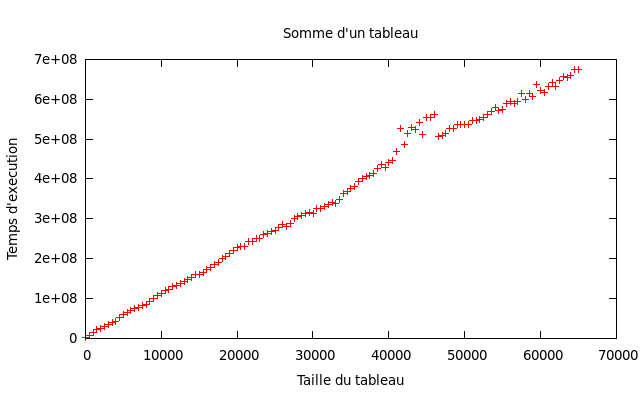
\includegraphics[width=0.9\textwidth]{arraysum.png}
\caption{Temps d'exécution des tests sur la somme des éléments d'un tableau}
\label{fig:arraysum}
\end{figure}
